\documentclass[11pt]{article}
\usepackage[margin=1in]{geometry}
\usepackage{upgreek}
\usepackage{xspace}
\usepackage{amsmath,amssymb}
\usepackage{graphicx}
\usepackage{booktabs}
\usepackage{tabularx}
\usepackage{caption}
\usepackage{enumitem}
\usepackage{xcolor}
\usepackage{listings}
\usepackage{verbatim}
\usepackage{needspace}
\usepackage{tikz}
\usetikzlibrary{arrows.meta,positioning}
\usepackage[framemethod=default]{mdframed}
\usepackage[hidelinks]{hyperref}
\captionsetup{font=small,labelfont=bf}
\setlength{\emergencystretch}{3em}
\setlist{itemsep=2pt,topsep=4pt}
\setlist[itemize]{label=$\bullet$}
\newcommand{\um}{\ensuremath{\,\upmu\mathrm{m}}\xspace}
\newcommand{\sbar}{\bar s}
\newcommand{\Dx}{D_x}
\newcommand{\Ical}{\mathcal{I}}
\newcommand{\code}[1]{\texttt{#1}}
\definecolor{boxgray}{gray}{0.95}
\definecolor{codegray}{gray}{0.965}
\newmdenv[backgroundcolor=boxgray,linewidth=0pt,innertopmargin=6pt,innerbottommargin=6pt,
  innerleftmargin=8pt,innerrightmargin=8pt,skipabove=8pt,skipbelow=8pt]{mathbox}
\newmdenv[backgroundcolor=white,linecolor=black!40,linewidth=0.6pt,innertopmargin=6pt,innerbottommargin=6pt,
  innerleftmargin=8pt,innerrightmargin=8pt,skipabove=8pt,skipbelow=8pt]{notebox}
\lstset{language=Python,basicstyle=\small\ttfamily,backgroundcolor=\color{codegray},frame=none,
  xleftmargin=6pt,xrightmargin=6pt,aboveskip=6pt,belowskip=6pt,columns=fullflexible,keepspaces=true,
  showstringspaces=false,commentstyle=\color{black!55},keywordstyle=\color{black}}

\title{\textbf{dsdfit}: Estimating Turbulent Broadening\\from Droplet Size Histograms\\[4pt]
\large A guide to the method, the code, and what to try}
\date{Version 0.1 \quad October 2026}

\begin{document}
\maketitle
\vspace{-1.5em}
\tableofcontents

%======================================================================
\section{What this is for}
%======================================================================

Clouds are made of water droplets of many different sizes. How widely those sizes spread out matters: a
broad spread of sizes is one of the first steps toward rain. One reason the sizes spread out is
turbulence. Different droplets experience different amounts of humidity as they are tossed around, so
they grow at different rates.

A model called the \emph{Fokker--Planck equation} describes this. It predicts the distribution of
droplet sizes from a few physical quantities. Two of them are hard to measure directly:
\begin{itemize}
\item $\sbar$, the \textbf{mean supersaturation}: on average, how much extra water vapor the air holds;
\item $\Dx$, the \textbf{broadening}: how strongly fluctuations in that humidity spread droplet sizes apart.
\end{itemize}
\textbf{dsdfit} estimates $\Dx$ and $\sbar$, with error bars, from a histogram of droplet sizes. It can
also make synthetic histograms from the model, so you can test the method before trusting it.

\begin{notebox}
\textbf{Your main task.} Simulations such as C-ODT (the Cloudy One-Dimensional Turbulence model) produce
droplet sizes \emph{and} record the humidity fluctuations that caused them. The model predicts
\begin{equation}
\Dx \approx a^2 \sigma_s^2\, \tau ,
\label{eq:Dx}
\end{equation}
where $\sigma_s$ measures how big the humidity fluctuations are and $\tau$ how long they last
(Section~\ref{sec:physics}). The task is to fit C-ODT size histograms with dsdfit and check whether the fitted
$\Dx$ agrees with $a^2\sigma_s^2\tau$ computed from C-ODT's own fluctuations (Section~\ref{sec:task}). If it
does, that is strong evidence that the method works on realistic data. If it does not, finding out why is
just as valuable.
\end{notebox}

%======================================================================
\section{The physics in plain words}\label{sec:physics}
%======================================================================

\paragraph{Supersaturation.} Air at a given temperature can hold only so much water vapor; at that point it
is \emph{saturated}. The \textbf{supersaturation} $s$ is how much extra vapor the air holds beyond
saturation, as a fraction: $s = 0.001$ means 0.1\% more vapor than saturation. When $s > 0$, water
condenses onto droplets and they grow; when $s < 0$, they evaporate. In clouds, $s$ is tiny, usually
well under 1\%. Throughout dsdfit, $s$ and $\sbar$ are written as fractions.

\paragraph{Droplets form on salt particles.} Droplets do not form from nothing: each one starts on a tiny
particle, here a grain of salt about $0.1\um$ across. Dissolved salt helps a small droplet take up water,
while the curvature of a very small droplet works against it. A droplet has to grow past a \emph{critical
size} before it can keep growing; this is called \emph{activation}. The size of the dry salt particle
matters for this step.

\paragraph{Growth.} Once activated, a droplet of radius $r$ grows as
\begin{equation}
\frac{d(r^2)}{dt} = a\,\big(s - s_{\rm eq}(r)\big),
\label{eq:growth}
\end{equation}
where $a$ is a \emph{growth constant} set by the temperature and pressure, and $s_{\rm eq}(r)$ is a small
correction from salt and curvature that only matters for the smallest droplets. Notice that it is the
\emph{square} of the radius that grows at a steady rate. That is why the model works with $x = r^2$.

\paragraph{Small droplets grow a little more slowly (optional).} Right at a droplet's surface, vapor and
heat are exchanged molecule by molecule, and not every vapor molecule that hits the surface sticks. This
slows small droplets by a factor $r/(r+\ell)$. The \emph{kinetic length} $\ell$ is set by two
\emph{accommodation coefficients}: $\alpha_c$, the fraction of vapor molecules that stick, and $\alpha_T$,
how well heat is passed to the air. By default dsdfit leaves this out ($\ell = 0$). To include it, give the
coefficients: \code{Conditions(alpha\_c=0.04, alpha\_T=1.0)} uses C-ODT's values, which give
$\ell \approx 1.5\um$ at 288\,K. Equation~\eqref{eq:growth} then becomes
\begin{equation*}
\frac{d(r+\ell)^2}{dt} = a\,\big(s - s_{\rm eq}(r)\big),
\end{equation*}
so the model works with $y = (r+\ell)^2$ instead of $r^2$, and nothing else changes. In particular,
$\Dx \approx a^2\sigma_s^2\tau$ still holds, now as the spreading of $y$.

\paragraph{Turbulence spreads sizes apart.} In turbulent air the supersaturation fluctuates around its mean
$\sbar$. The size of the fluctuations is measured by their standard deviation $\sigma_s$, and how long a
typical fluctuation lasts by a time scale $\tau$. Each droplet experiences its own random sequence of
fluctuations, so identical droplets end up with different sizes. In the model this spreading acts like
diffusion in $x$, with strength $\Dx$; if the fluctuations are brief compared with the time a droplet takes
to grow, then $\Dx \approx a^2\sigma_s^2\tau$, which is equation~\eqref{eq:Dx}.

\paragraph{Falling out.} Bigger droplets fall faster: the falling speed is proportional to $r^2$. In a
well-mixed chamber of height $H$, droplets of radius $r$ are removed at a rate $k r^2$, where the
\emph{fallout constant} $k$ is set by the falling speed and the chamber height.

\paragraph{Steady state.} New particles are injected continuously, grow, spread apart, and eventually fall
out. When these processes balance, the size distribution stops changing. The model predicts this
\emph{steady} distribution (Figure~\ref{fig:schematic}).

\begin{figure}[h]
\centering
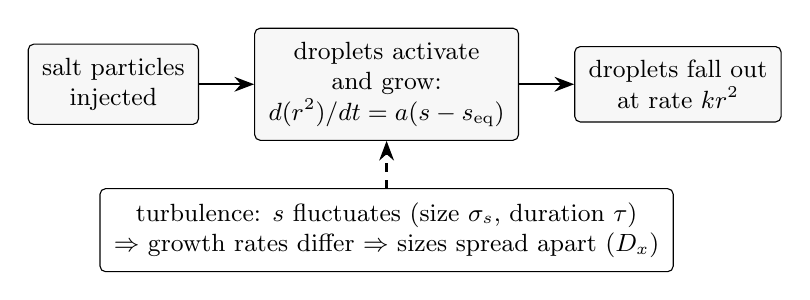
\begin{tikzpicture}[node distance=7mm, every node/.style={font=\small},
  box/.style={draw, rounded corners=2pt, align=center, inner sep=5pt, fill=black!3},
  arr/.style={-{Stealth[length=2.5mm]}, thick}]
\node[box] (inj) {salt particles\\injected};
\node[box, right=of inj] (grow) {droplets activate\\and grow:\\$d(r^2)/dt = a(s - s_{\rm eq})$};
\node[box, right=of grow] (fall) {droplets fall out\\at rate $k r^2$};
\node[box, below=6mm of grow, fill=white] (turb) {turbulence: $s$ fluctuates (size $\sigma_s$, duration $\tau$)\\
$\Rightarrow$ growth rates differ $\Rightarrow$ sizes spread apart ($\Dx$)};
\draw[arr] (inj) -- (grow);
\draw[arr] (grow) -- (fall);
\draw[arr, dashed] (turb) -- (grow);
\end{tikzpicture}
\caption{The life of a droplet in the model. In steady state, injection, growth, spreading and fallout
balance, and the size distribution no longer changes.}
\label{fig:schematic}
\end{figure}

\paragraph{The model.} Writing $N(x)$ for the number of droplets per unit $x = r^2$, the steady
Fokker--Planck equation is
\begin{mathbox}
\begin{equation}
\frac{d}{dx}\Big[\,\underbrace{a\Big(\sbar - \frac{A_k}{r} + \frac{B_k}{r^3}\Big)N}_{\text{growth}}
\;-\; \underbrace{\Dx\,\frac{dN}{dx}}_{\text{spreading}}\Big]
\;+\; \underbrace{k\,x\,N}_{\text{falling out}} \;=\; 0 .
\label{eq:fp}
\end{equation}
\end{mathbox}
The bracket is the rate at which droplets move toward larger sizes. Droplets are injected at the smallest
size and none go past the largest. With the kinetic correction, $x$ is replaced by $y = (r+\ell)^2$; the
fallout term stays $k r^2 N$. You will not need to solve this yourself; dsdfit does it.

\paragraph{The parameters.} Table~\ref{tab:params} lists everything that enters. The first two are
estimated; the next two are what C-ODT can provide for the comparison; the rest you set to match your
data, and dsdfit computes the model constants from them.

\begin{table}[h]
\centering\small
\begin{tabularx}{\textwidth}{l X l l l}
\toprule
Symbol & Meaning & Units & Example & In dsdfit \\
\midrule
$\sbar$ & mean supersaturation & fraction & 0.0009 & \textbf{estimated} (\code{s\_bar}) \\
$\Dx$ & how strongly fluctuations spread sizes & $\upmu$m$^4$/s & 0.3 & \textbf{estimated} (\code{D\_x}) \\
\midrule
$\sigma_s$ & size of the supersaturation fluctuations & fraction & 0.002 & from C-ODT, for comparison \\
$\tau$ & how long a fluctuation lasts & s & 2 & from C-ODT, for comparison \\
\midrule
$T$ & air temperature & K & 288 & \code{Conditions(T=...)} \\
$p$ & air pressure & Pa & $1.0\times10^5$ & \code{Conditions(p=...)} \\
$d_{\rm dry}$ & diameter of the dry salt particle & $\upmu$m & 0.13 & \code{Conditions(d\_dry=...)} \\
$H$ & chamber height & m & 1 & \code{Conditions(H=...)} \\
$\alpha_c$, $\alpha_T$ & accommodation coefficients (optional) & fraction & 0.04, 1 & \code{Conditions(alpha\_c=...)} \\
\midrule
$a$ & growth constant & $\upmu$m$^2$/s & 206 & computed (\code{cond.a}) \\
$A_k$, $B_k$ & curvature and salt constants & $\upmu$m, $\upmu$m$^3$ & & computed \\
$k$ & fallout constant & s$^{-1}\upmu$m$^{-2}$ & $1.2\times10^{-4}$ & computed (\code{cond.k}) \\
$\ell$ & kinetic length & $\upmu$m & 0 & computed (\code{cond.ell}) \\
\bottomrule
\end{tabularx}
\caption{The parameters. Example values are the defaults used in this guide. The accommodation coefficients
are not set by default ($\ell = 0$); 0.04 and 1 are C-ODT's values.}
\label{tab:params}
\end{table}

\needspace{8\baselineskip}
\paragraph{What a histogram can and cannot tell you.}
\begin{itemize}
\item It tells you the \textbf{shape} of the distribution, which depends on $\Dx$ and $\sbar$
(Figure~\ref{fig:params}). It does not depend on how many particles were injected.
\item It \textbf{cannot separate $\sigma_s$ from $\tau$}: they only enter through $\Dx$. That is why the
comparison uses their combination $a^2\sigma_s^2\tau$.
\item It relies on the growth constant $a$ and fallout constant $k$ being right. If the conditions you give
are wrong, the estimates will be off. The fit check (Section~\ref{sec:method}) can sometimes tell you.
\end{itemize}

\begin{figure}[h]
\centering
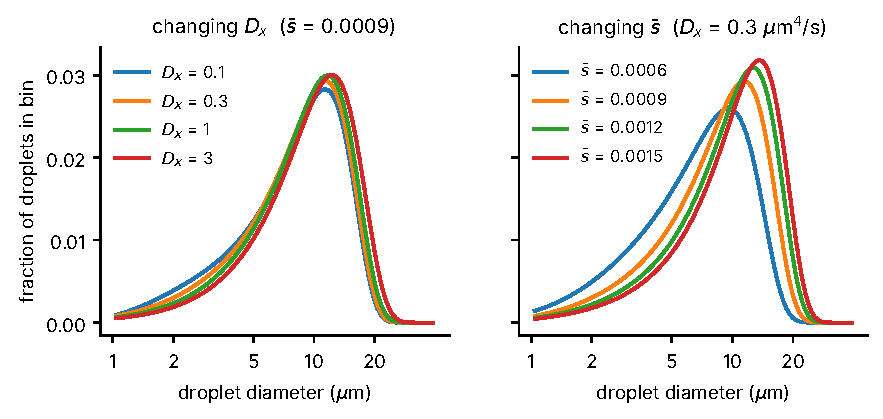
\includegraphics[width=\textwidth]{figs/what_params_do.pdf}
\caption{The model's predicted fraction of droplets in each bin. Raising $\Dx$ (left) or $\sbar$ (right)
both move droplets toward larger sizes, in somewhat different ways. Because the effects are similar, the
two estimates end up correlated.}
\label{fig:params}
\end{figure}

%======================================================================
\section{What the method does}\label{sec:method}
%======================================================================

\paragraph{The data.} A histogram records how many droplets fell in each size bin. It carries two separate
pieces of information: the \emph{shape} (what fraction of droplets is in each bin) and the \emph{number of
droplets} $n$. The model predicts the shape. The number of droplets tells you how noisy the histogram is:
a histogram of 100 droplets is ragged, one of 100{,}000 is smooth.

\paragraph{The fit.} \code{fit} tries values of $\Dx$ and $\sbar$, computes the predicted fractions, and
measures the mismatch with the observed counts with a number $J$ (the \emph{loss}). It searches for the
pair that makes $J$ smallest. That pair is the estimate. How the mismatch is measured and how the search
works are in Appendix~\ref{app:how}; you do not need them to use the code.

\paragraph{Error bars.} Each estimate comes with an error bar of one standard deviation. If you repeated
the experiment many times, the estimate would land within one error bar of the true value about 2 times
in 3, and within two error bars about 19 times in 20. Error bars shrink as the number of droplets grows.
\code{fit} also reports the \emph{correlation} between the two estimates. It is usually strongly
negative: a histogram that slightly favors a larger $\Dx$ also favors a smaller $\sbar$, because the two
have similar effects (Figure~\ref{fig:params}).

\paragraph{The fit check.} Even with the true parameters, a histogram never matches the model exactly,
because of counting noise. dsdfit knows roughly how large $J$ should be when the model is right
(\code{J\_expected}) and compares it with the value at the best fit (\code{J\_min}). If \code{J\_min} is
much larger, the model cannot describe the data: the conditions may be wrong, or the data may break one of
the model's assumptions.

\paragraph{Assumptions.} The method assumes
(1) the distribution is in steady state;
(2) each droplet is counted once and independently of the others;
(3) every droplet in the histogram's size range is counted equally well; and
(4) the conditions (temperature, pressure, particle size, chamber height) are right.

\begin{figure}[h]
\centering
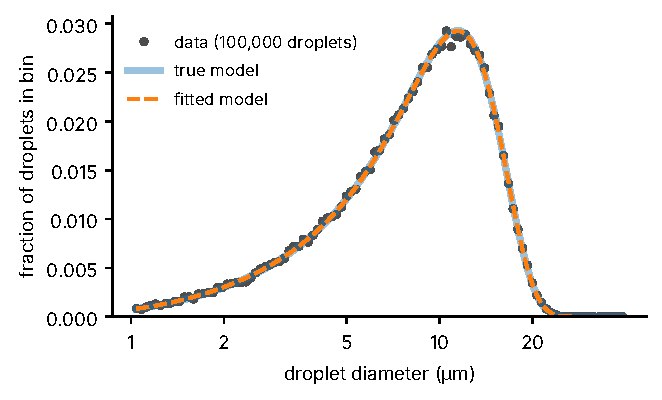
\includegraphics[width=0.62\textwidth]{figs/one_fit.pdf}

\vspace{4pt}
\begin{minipage}{0.86\textwidth}
\footnotesize
\verbatiminput{figs/one_fit_summary.txt}
\end{minipage}
\caption{One synthetic histogram of $10^5$ droplets (true $\Dx = 0.3$, $\sbar = 0.0009$), the fitted model,
and the summary printed by \code{print(result)}.}
\label{fig:onefit}
\end{figure}

%======================================================================
\section{Using the code}\label{sec:code}
%======================================================================

\subsection{Installing}
\begin{lstlisting}[language=bash]
git clone https://github.com/dawsoncollins99/dsdfit.git
cd dsdfit
pip install -e ".[notebook]"
\end{lstlisting}
Then open \code{examples/example.ipynb}, which walks through everything in this section.

\subsection{The functions}

\begin{center}\small
\begin{tabularx}{\textwidth}{l X}
\toprule
Function & What it does \\
\midrule
\code{Conditions(T, p, d\_dry, H, alpha\_c, alpha\_T)} & physical conditions; computes $a$, $A_k$, $B_k$, $k$, $\ell$ (\code{print(cond)} shows them) \\
\code{welas\_bins(cutoff\_diameter=1.0)} & bin edges of the WELAS instrument: 103 bins from 1 to 40\um \\
\code{Histogram(edges, counts)} & droplet counts in size bins (Section~\ref{sec:format}) \\
\code{load\_histogram(path)}, \code{save\_histogram(h, path)} & read and write histograms as CSV files \\
\code{model\_fractions(D\_x, s\_bar, cond, edges)} & the model's predicted fraction of droplets in each bin \\
\code{simulate(D\_x, s\_bar, cond, edges, n, seed)} & a synthetic histogram of \code{n} droplets \\
\code{model\_evolution(D\_x, s\_bar, cond, edges, times)} & droplet numbers in each bin over time, after a pulse of aerosol or from an empty chamber \\
\code{fit(hist, cond)} & estimates of $\Dx$ and $\sbar$ with error bars, as a \code{FitResult} \\
\code{predicted\_D\_x(sigma\_s, tau, cond)} & $a^2\sigma_s^2\tau$, to compare with a fitted $\Dx$ \\
\code{plot\_fit(hist, result)} & plot a histogram with the true and fitted model \\
\bottomrule
\end{tabularx}
\end{center}

A \code{FitResult} has the attributes \code{D\_x}, \code{D\_x\_err}, \code{s\_bar}, \code{s\_bar\_err},
\code{correlation}, \code{J\_min}, \code{J\_expected}, \code{fit\_ok}, \code{n}, \code{converged} and
\code{fractions} (the fitted model's fraction in each bin).

\begin{notebox}
\textbf{Conventions.} Sizes you type are droplet \textbf{diameters in micrometers}. $\Dx$ is in
$\upmu$m$^4$/s. $\sbar$ and $\sigma_s$ are \textbf{fractions} (0.0009 means 0.09\%). Times are in seconds.
\end{notebox}

\subsection{The histogram format}\label{sec:format}

Everything \code{fit} needs from the data is a histogram: bin edges and counts. In Python,
\code{Histogram(edges, counts)}; on disk, a CSV file with one row per bin:
\begin{lstlisting}[language={}]
# comment lines start with #
lower_diameter_um,upper_diameter_um,count
1.0233,1.06038,88
1.06038,1.0988,75
...
\end{lstlisting}
The rules:
\begin{itemize}
\item \textbf{Edges are diameters in $\upmu$m}, strictly increasing. Bins must be contiguous: each upper edge
is the next bin's lower edge. Bins do not have to be the WELAS bins.
\item \textbf{Counts are whole numbers of droplets}, one per bin. A normalized distribution, a
concentration, or a probability density is \emph{not} a valid set of counts. \code{Histogram} refuses
non-whole numbers.
\item \textbf{Each droplet is counted once, independently.} The error bars depend on this. If you add up
many snapshots of a simulation that contain the same droplets, each droplet is counted many times: the
estimates are still fine, but the error bars will be too small.
\item \textbf{Use plenty of droplets.} dsdfit warns below 10{,}000; with fewer, error bars are less reliable.
\end{itemize}

\needspace{14\baselineskip}
\subsection{Examples}

\paragraph{Simulate and fit.} This produces Figure~\ref{fig:onefit}.
\begin{lstlisting}
from dsdfit import Conditions, welas_bins, simulate, fit, plot_fit

cond  = Conditions()            # T = 288 K, p = 1e5 Pa, d_dry = 0.13 um, H = 1 m
edges = welas_bins()            # 103 bins from 1 to 40 um
hist  = simulate(D_x=0.3, s_bar=0.0009, cond=cond, edges=edges, n=100_000, seed=1)
result = fit(hist, cond)
print(result)
plot_fit(hist, result)
\end{lstlisting}

\paragraph{Does it recover the truth?} Repeat with different random seeds and compare the estimates with
the true values (Figure~\ref{fig:recovery}). The notebook contains the plotting code.
\begin{lstlisting}
results = [fit(simulate(0.3, 0.0009, cond, edges, n=100_000, seed=s), cond)
           for s in range(20)]
\end{lstlisting}

\begin{figure}[h]
\centering
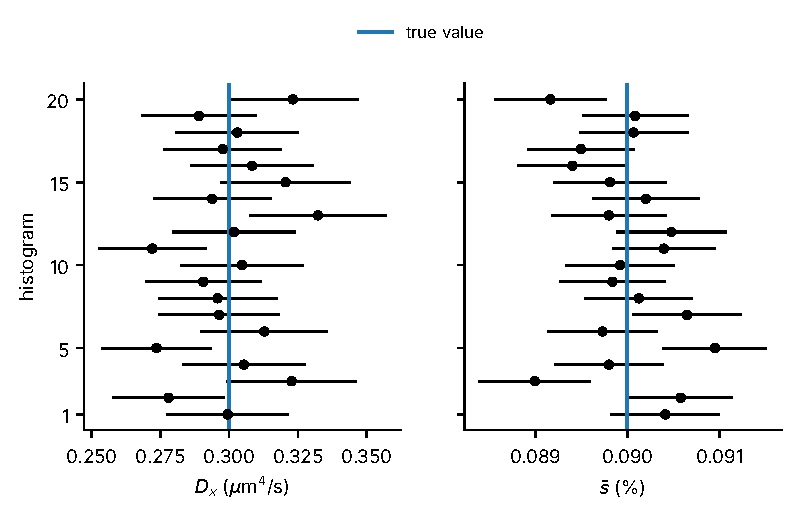
\includegraphics[width=0.82\textwidth]{figs/recovery.pdf}
\caption{Twenty synthetic histograms of $10^5$ droplets each, fitted with the same conditions that made
them. The true value lies within one error bar for 16 of the 20 $\Dx$ estimates and 14 of the 20 $\sbar$
estimates, and within two error bars for all of them, as expected.}
\label{fig:recovery}
\end{figure}

\needspace{7\baselineskip}
\paragraph{Fitting with different conditions.} The conditions used to \emph{make} the data and the
conditions the fit \emph{assumes} are separate arguments, so you can ask what happens when the fit assumes
something slightly wrong:
\begin{lstlisting}
hist = simulate(0.3, 0.0009, Conditions(H=1.0), edges, n=100_000, seed=1)
result = fit(hist, Conditions(H=1.1))       # the fit assumes a chamber 10% taller
\end{lstlisting}

\needspace{8\baselineskip}
\paragraph{Data from a file.} This is how other data, such as a C-ODT histogram, come in:
\begin{lstlisting}
from dsdfit import load_histogram, predicted_D_x
hist = load_histogram("data/example_histogram.csv")
result = fit(hist, cond)
D_pred = predicted_D_x(sigma_s=0.0019, tau=2.0, cond=cond)
print((result.D_x - D_pred) / result.D_x_err, "error bars apart")
\end{lstlisting}

%======================================================================
\section{The main task: C-ODT}\label{sec:task}
%======================================================================

The goal is to find out whether the fitted $\Dx$ agrees with $a^2\sigma_s^2\tau$ computed from C-ODT's
supersaturation record. Here is one way to go about it.

\begin{enumerate}[itemsep=4pt]
\item \textbf{Pick a steady period.} After a simulation starts, the size distribution takes a while to
settle. Use only output after it has stopped changing (compare histograms from early and late in the
period).
\item \textbf{Build the histogram.} Count droplets in diameter bins and write the CSV file
(Section~\ref{sec:format}). You can use the WELAS bins, to mimic the instrument, or your own bins over all
sizes. Make sure each count is a number of droplets, and think about whether the same droplets appear in
several of the snapshots you combine.
\item \textbf{Set the conditions.} Use the run's temperature, pressure, dry particle size and domain
height. C-ODT includes the kinetic correction with $\alpha_c = 0.04$ and $\alpha_T = 1$, so pass those too.
Check how C-ODT removes droplets: dsdfit assumes they fall out at rate $k r^2$, with $k$ set by the
chamber height.
\item \textbf{Fit.} Look at the estimates, the error bars, and the fit check. Plot the histogram with the
fitted model.
\item \textbf{Compute $\sigma_s$ and $\tau$} from the supersaturation experienced by droplets over the same
period. With $s'(t) = s(t) - \sbar$ the fluctuation,
\begin{equation*}
\sigma_s^2 = \text{average of } s'^2,
\qquad
\rho(t) = \frac{\text{average of } s'(t_0)\,s'(t_0 + t)}{\sigma_s^2},
\qquad
\tau = \int_0^{\infty} \rho(t)\,dt .
\end{equation*}
$\rho(t)$ is the autocorrelation: how similar the supersaturation is to itself a time $t$ later. It
starts at 1 and decays; $\tau$ is the area under it. In practice, integrate until $\rho$ first drops to
zero.
\item \textbf{Compare.} Compute \code{predicted\_D\_x(sigma\_s, tau, cond)} and compare it with the fitted
$\Dx$, in units of the error bar. Also compare the fitted $\sbar$ with C-ODT's mean supersaturation.
\end{enumerate}

\paragraph{If they disagree.} Some possible reasons, each worth checking:
\begin{itemize}
\item the conditions do not match the run (especially anything affecting growth or fallout);
\item the histogram includes particles that have not activated, which the model's spreading term cannot
describe (with 0.13\um\ salt particles, activation happens near 2\um\ diameter; try \code{welas\_bins(3.0)});
\item the period is not steady, or the counts are not independent (error bars too small);
\item C-ODT injects or removes droplets differently from the model;
\item the fluctuations last too long for $\Dx \approx a^2\sigma_s^2\tau$ to hold (it needs $\tau$ short
compared with the time a droplet takes to grow);
\item $\sigma_s$ and $\tau$ were computed from supersaturation at fixed points in space rather than as
experienced by the droplets.
\end{itemize}

%======================================================================
\section{Suggested warm-ups}\label{sec:warmups}
%======================================================================

Before working with C-ODT data, a few experiments with synthetic data will help you know what to expect.
For each, predict the answer before running it.
\begin{itemize}
\item \textbf{Recovery at your run's conditions.} Repeat the recovery experiment of
Figure~\ref{fig:recovery} with the C-ODT run's conditions and plausible values of $\Dx$ and $\sbar$.
\item \textbf{More droplets.} How do the error bars change as $n$ goes from $10^3$ to $10^6$? Plot them on
log--log axes.
\item \textbf{Wrong conditions.} Simulate with one set of conditions and fit with another (for example, a
chamber height 10\% off). How far off are the estimates, measured in error bars? Does the fit check notice?
\item \textbf{The detection limit.} Compare \code{welas\_bins(1.0)}, \code{welas\_bins(2.0)} and bins
covering all sizes. How much do the error bars change?
\end{itemize}

\appendix

%======================================================================
\section{Glossary}
%======================================================================
\begin{description}[itemsep=2pt,font=\normalfont\bfseries]
\item[Activation] a droplet growing past its critical size, after which it keeps growing.
\item[Autocorrelation] how similar a fluctuating quantity is to itself a time $t$ later.
\item[Correlation (of estimates)] how much an error in one estimate tends to come with an error in the
other; between $-1$ and $1$.
\item[Error bar] here, one standard deviation of the estimate.
\item[Fallout] droplets settling out of the chamber under gravity.
\item[Fokker--Planck equation] an equation for how a distribution changes under drift (here, growth),
diffusion (here, spreading by turbulence) and removal.
\item[Histogram] counts of droplets in size bins.
\item[Steady state] a situation where the distribution no longer changes in time.
\item[Supersaturation] how much water vapor the air holds beyond saturation, as a fraction.
\end{description}

%======================================================================
\section{How the fit works}\label{app:how}
%======================================================================

This appendix is for anyone curious about what happens inside \code{fit}. Notation: the histogram has
counts $c_k$ in bins $k = 1,\dots,K$, with $n = \sum_k c_k$ droplets; $p_k(\theta)$ is the model's fraction
in bin $k$; and $\theta = (\ln\Dx, \sbar)$.

\paragraph{Solving the model.} Equation~\eqref{eq:fp} is solved with finite volumes on a fine, uniform grid
in $y = (r+\ell)^2$ (that is, $x = r^2$ when $\ell = 0$), using Scharfetter--Gummel fluxes, which stay accurate whether growth or spreading dominates.
The result is one tridiagonal linear system. The solution is summed over each bin and normalized to give
$p_k$.

\paragraph{The loss.} If each droplet lands in bin $k$ with probability $p_k$, independently of the others,
the probability of the observed counts is proportional to $\prod_k p_k^{c_k}$. Maximizing it is the same as
minimizing
\begin{equation}
J(\theta) = 2\sum_k c_k \ln\frac{c_k}{n\,p_k(\theta)} ,
\end{equation}
which is zero only if the model matches the histogram exactly. For large counts,
$J \approx \sum_k (c_k - n p_k)^2/(n p_k)$: a least-squares mismatch in which each bin is weighted by
its expected noise.

\paragraph{The search (Gauss--Newton).} Starting from the best of a coarse grid of precomputed shapes,
each step solves a $2\times2$ linear system,
\begin{equation}
n\,\Ical\,\Delta\theta = \sum_k \frac{c_k - n p_k}{p_k}\,\frac{\partial p_k}{\partial\theta},
\qquad
\Ical_{ij} = \sum_k \frac{1}{p_k}\,\frac{\partial p_k}{\partial\theta_i}\,\frac{\partial p_k}{\partial\theta_j},
\end{equation}
and moves along $\Delta\theta$: it tries the full step and the bottom of a parabola fitted to $J$ along the
step, keeps whichever gives the lower $J$, and halves the step if $J$ still does not go down (a very long
step is capped first). $\Delta\theta$ is the step that would
fit the current mismatch exactly if the model were linear near $\theta$. It usually converges in a handful
of steps. The derivatives $\partial p_k/\partial\theta$ come from two more solves of the same tridiagonal
system (the \emph{tangent-linear} method).

\paragraph{Error bars.} The matrix $\Ical$ is the \emph{Fisher information}: how much one droplet tells
you about $\theta$. With $n$ droplets, the covariance of the estimates is
\begin{equation}
\Sigma = (n\,\Ical)^{-1},
\end{equation}
so the error bar on $\ln\Dx$ is $\sqrt{\Sigma_{11}}$ (a relative error on $\Dx$), the error bar on $\sbar$
is $\sqrt{\Sigma_{22}}$, and their correlation is $\Sigma_{12}/\sqrt{\Sigma_{11}\Sigma_{22}}$. These
formulas assume many droplets and independent counts.

\paragraph{The fit check.} When the model is right, $J_{\min}$ behaves roughly like a sum of one squared,
standardized error per bin, so its typical value is about the number of well-populated bins minus 3 (one for
the fixed total and one for each estimated parameter), with a spread of about $\sqrt{2\,J_{\rm expected}}$.
\code{fit\_ok} is true when $J_{\min}$ is within three spreads of that value.


%======================================================================
\section{Troubleshooting}
%======================================================================
\begin{description}[itemsep=4pt,font=\normalfont\bfseries]
\item[``counts must be whole numbers of droplets''] The data are a normalized distribution or a
concentration. Convert them to the number of independent droplets they represent.
\item[``Histogram has only \dots\ droplets''] A warning, not an error: with fewer than about 10{,}000
droplets, the error bars are less reliable.
\item[\code{fit\_ok} is False] The model does not describe the data well. Check the conditions, whether the
data are in steady state, and whether the counts are independent.
\item[\code{converged} is False] Try a starting guess close to where you expect the answer:
\code{fit(hist, cond, start=(D\_x, s\_bar))}.
\item[Very large error bars, correlation near $\pm1$] The histogram cannot tell $\Dx$ and $\sbar$ apart in
this situation; more droplets, or bins covering more sizes, may help.
\item[``The model puts (almost) no droplets in the bins''] The bins lie where the model predicts no
droplets (for example, all far beyond the largest droplets), or the parameters are extreme.
\item[``needs too fine a grid''] The bins extend to very large sizes. Drop empty bins far beyond the
largest droplets.
\end{description}

\end{document}
